%--------------------------------------------------------------------%
%
% Berkas utama templat LaTeX.
%
% author Petra Barus, Peb Ruswono Aryan
%
%--------------------------------------------------------------------%
%
% Berkas ini berisi struktur utama dokumen LaTeX yang akan dibuat.
%
%--------------------------------------------------------------------%

\documentclass[12pt, a4paper, onecolumn, oneside, final]{report}

% Default fixed font does not support bold face
\DeclareFixedFont{\ttb}{T1}{txtt}{bx}{n}{12} % for bold
\DeclareFixedFont{\ttm}{T1}{txtt}{m}{n}{12}  % for normal

% custom colors
\usepackage{color}
\definecolor{deepblue}{rgb}{0,0,0.5}
\definecolor{deepred}{rgb}{0.6,0,0}
\definecolor{deepgreen}{rgb}{0,0.5,0}

\usepackage{listings}
\usepackage{amsmath}
\newcommand\numberthis{\addtocounter{equation}{1}\tag{\theequation}}

% Python style for highlighting
\newcommand\pythonstyle{\lstset{
language=Python,
basicstyle=\ttm,
otherkeywords={}, % tambah disini buat highlight biru (fungsi internal python: def, print, dll)
keywordstyle=\ttb\color{deepblue},
emph={},          % buat highlight merah (gatau buat apa ya wkwk, kalo mau isi nama2 library paling)
emphstyle=\ttb\color{deepred},    % Custom highlighting style
stringstyle=\color{deepgreen},
frame=tb,                         % Any extra options here
showstringspaces=false            % 
}}

% Python environment
\lstnewenvironment{python}[1][]
{
\pythonstyle
\lstset{#1}
}
{}

% Python for inline
\newcommand\pythoninline[1]{{\pythonstyle\lstinline!#1!}}


%-------------------------------------------------------------------%
%
% Konfigurasi dokumen LaTeX untuk laporan tesis IF ITB
%
% @author Petra Novandi
%
%-------------------------------------------------------------------%
%
% Berkas asli berasal dari Steven Lolong
%
%-------------------------------------------------------------------%

% Ukuran kertas
\special{papersize=210mm,297mm}

% Setting margin
\usepackage[top=3cm,bottom=2.5cm,left=4cm,right=2.5cm]{geometry}

\usepackage{mathptmx}

% Judul bahasa Indonesia
\usepackage[bahasa]{babel}

% Format citation
\usepackage[backend=bibtex,citestyle=numeric]{biblatex}

\usepackage[utf8]{inputenc}
\usepackage{graphicx}
\usepackage{titling}
\usepackage{blindtext}
\usepackage{sectsty}
\usepackage{chngcntr}
\usepackage{etoolbox}
\usepackage{hyperref}       % Package untuk link di daftar isi.
\usepackage{titlesec}       % Package Format judul
\usepackage{parskip}

% Line satu setengah spasi
\renewcommand{\baselinestretch}{1.5}

% Setting judul
\chapterfont{\centering \Large}
\titleformat{\chapter}[display]
  {\Large\centering\bfseries}
  {\chaptertitlename\ \thechapter}{0pt}
    {\Large\bfseries\uppercase}

% Setting nomor pada subbsubsubbab
\setcounter{secnumdepth}{3}

\makeatletter

\makeatother

% Counter untuk figure dan table.
\counterwithin{figure}{section}
\counterwithin{table}{section}


\makeatletter

\makeatother

\bibliography{references}

\begin{document}

    %Basic configuration
    \title{Analisis Metode LSTM Autoencoder dan Bayesian Probability untuk Anomaly Detection}
    \date{}
    \author{
        Saleh Zaidan \quad 13318006 \\
        Farrel Dzaudan Naufal \quad 13318048
    }

    \pagenumbering{roman}
    \setcounter{page}{0}

    \clearpage
\pagestyle{empty}

\begin{center}
\smallskip

    \Large \bfseries \MakeUppercase{\thetitle}
    \vfill

    \Large Laporan Tugas Besar \\ TF4063 Sains Data Rekayasa \\ Semester I 2020/2021
    \vfill

    %\large Disusun sebagai syarat kelulusan tingkat sarjana
    %\vfill

    \large Oleh

    \Large \theauthor

    \vfill
    \begin{figure}[h]
        \centering
      	\includegraphics[width=0.25\textwidth]{resources/cover-ganesha.jpg}
    \end{figure}
    \vfill

    \large
    \uppercase{
        Program Studi Teknik Fisika \\
        Fakultas Teknologi Industri \\
        Institut Teknologi Bandung
    }

    2020

\end{center}

\clearpage

    %\input{chapters/approval}
    %\input{chapters/statement}

    \pagestyle{plain}

    %\input{chapters/abstract-id}
    %\input{chapters/abstract-en}
    %\input{chapters/forewords}

    \titleformat*{\section}{\centering\bfseries\Large\MakeUpperCase}

    \tableofcontents
    %\listoffigures
    %\listoftables

    \titleformat*{\section}{\bfseries\Large}
    \pagenumbering{arabic}

    %----------------------------------------------------------------%
    % Konfigurasi Bab
    %----------------------------------------------------------------%
    \setcounter{page}{1}
    \renewcommand{\chaptername}{BAB}
    \renewcommand{\thechapter}{\Roman{chapter}}
    %----------------------------------------------------------------%

    %----------------------------------------------------------------%
    % Dafter Bab
    % Untuk menambahkan daftar bab, buat berkas bab misalnya `chapter-6` di direktori `chapters`, dan masukkan ke sini.
    %----------------------------------------------------------------%
    \chapter{Pendahuluan}

\section{Prelude: Preventative Maintenance for Machine Failure}

\section{Anomaly Detection: An Unsupervised Learning}

    \chapter{Metode Acuan}

\section{Latar Belakang Data}

Data yang digunakan adalah data pembacaan sensor pada pompa air yang berasal dari seorang pengguna di Kaggle \cite{pump_sensor_data}. Pompa air yang digunakan sering mengalami kerusakan sehingga menimbulkan permasalahan serius terhadap kehidupan warga. Tim yang bekerja tidak dapat melihat pola apapun pada data ketika sistem rusak, sehingga diharapkan dapat ditemukan suatu cara untuk memprediksinya.

\section{Data Preprocessing}

Data terdiri dari 220.320 entri yang terbagi dalam 3 grup utama:

\begin{enumerate}
    \item Timestamp
    \item Sensor
    \item Status mesin: Label target yang diprediksi ketika kerusakan akan terjadi
\end{enumerate}

Timestamp tertulis dalam format: \texttt{tahun-bulan-tanggal jam:menit:detik}

Sensor tersebar dalam 52 kolom dari \texttt{sensor\_00} hingga \texttt{sensor\_51} yang terdiri dari nilai float.

Status mesin terdiri dari 3 kelas: NORMAL, BROKEN, dan RECOVERING yang masing-masing menyatakan kondisi normal, rusak, dan pulih pada pompa.

    \subsection{Data Cleaning}

    Terdapat beberapa hal yang harus dilakukan terlebih dahulu pada data:

    \begin{enumerate}
        \item Menghapus kolom berlebih
        \item Menghapus duplikat
        \item Mengatasi nilai yang hilang (not available/NA)
        \item Mengkonversi tipe data ke tipe yang benar
    \end{enumerate}
    
    Untuk mengatasi nilai hilang dicari 10 sensor dengan jumlah NA terbanyak. Kemudian NA pada sensor tersebut diisi oleh nilai mean-nya (impute), sedangkan NA pada sensor lain dihapus.

    \subsection{Dimensional Reduction}

    Komputasi dengan seluruh kolom dari sensor akan membutuhkan waktu yang lama dan tidak efisien. Sehingga diterapkan principal component analysis (PCA) untuk menghasilkan fitur baru yang dapat digunakan pada modeling. Namun sebelum itu data perlu diskala terlebih dahulu karena PCA merupakan algoritma berbasis jarak. Jika dilihat pada 10 data pertama besar nilai bacaan tidak konsisten pada tiap sensor, beberapa sangat besar dan yang lain justru sangat kecil.

        \subsubsection{Principal Component Analysis}

        \begin{figure}[h]
            % \centering
            \centerline{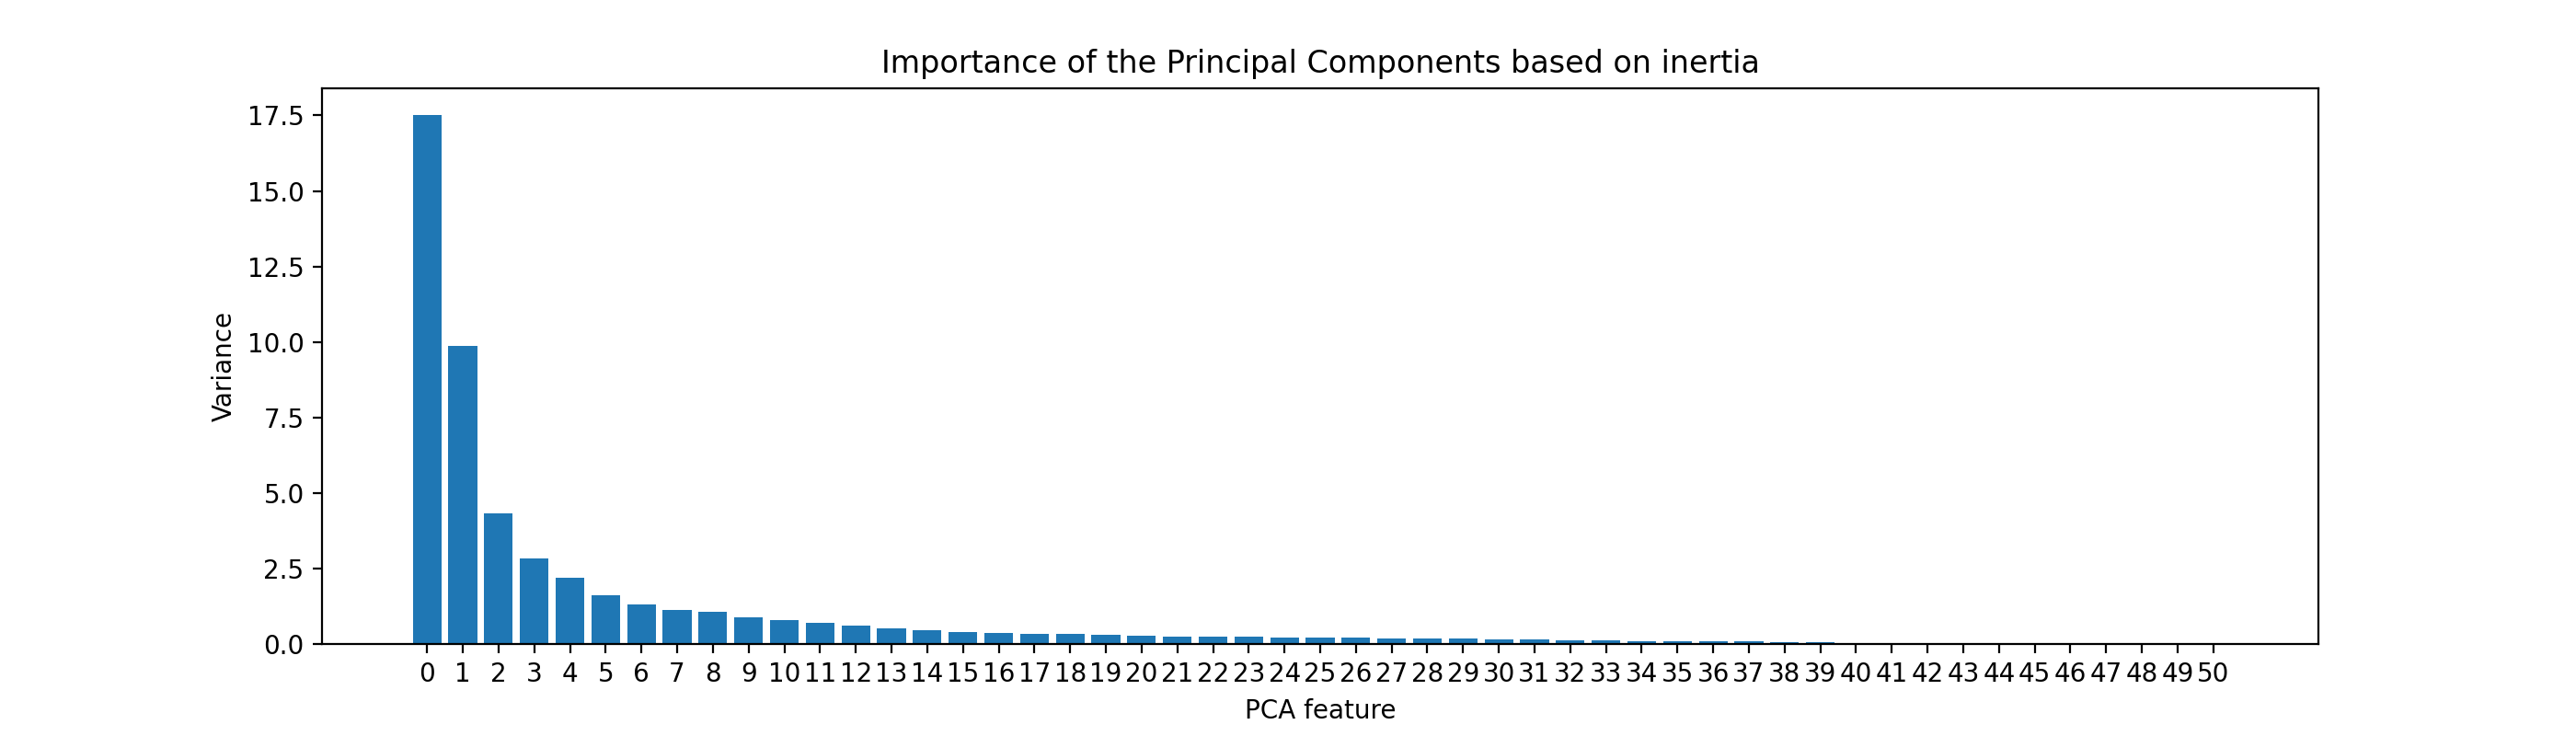
\includegraphics[width=1.2\textwidth]{resources/Acuan/PCA_Plot.png}}
            \caption{Komponen Utama PCA}
        \end{figure}

        Setelah dianalisis berdasarkan nilai variansi ternyata 2 komponen utama pertama adalah yang paling penting, sehingga PCA dilakukan dengan menggunakan 2 komponen tersebut yang kemudian digunakan pada pelatihan model.

        \subsubsection{Stationarity and Autocorrelation}

        Stationarity merupakan perilaku data time-series saat nilai mean dan standar deviasinya tidak berubah sepanjang waktu. Sedangkan autocorrelation merupakan perilaku data ketika terkorelasi dengan dirinya sendiri pada periode waktu yang berbeda.

        Untuk mengecek stationarity secara kuantitatif dilakukan Augmented Dickey-Fuller Test pada kedua komponen utama dari PCA.

\begin{python}
from statsmodels.tsa.stattools import adfuller
# Run Augmented Dickey Fuller Test
result = adfuller(principalDf['pc1'])
# Print p-value
print(result[1])
# Out : 5.453684941848713e-05

# Run Augmented Dickey Fuller Test
result = adfuller(principalDf['pc2'])
# Print p-value
print(result[1])
# Out : 1.8909142426286498e-06
\end{python}

        Untuk mengecek autocorrelation digunakan plot ACF (autocorrelation function) untuk memperoleh hasil secara visual.

\begin{python}
# Compute change in daily mean 
pca1 = principalDf['pc1'].pct_change()
# Compute autocorrelation
autocorrelation = pca1.dropna().autocorr()
print('Autocorrelation is: ', autocorrelation)
# Out : Autocorrelation is -0.002051194822378389

# Compute change in daily mean 
pca2 = principalDf['pc2'].pct_change()
# Compute autocorrelation
autocorrelation = pca2.autocorr()
print('Autocorrelation is: ', autocorrelation)
# Out : Autocorrelation is -3.150648347070906e-05
\end{python}

\section{Modeling}

    \subsection{Interquartile Range (IQR)}

    Strategi dari model ini adalah: \cite{metode_acuan}

    \begin{enumerate}
        \item Hitung nilai IQR, yaitu beda dari persentil ke-75 (Q3) dan ke-25 (Q1)
        \item Hitung batas atas dan bawah untuk outlier
        \item Filter data yang berada di atas dan di bawah batas dan tandai sebagai outlier
        \item Plot outlier di atas data time-series
    \end{enumerate}

\begin{python}
# Calculate IQR for the 1st principal component (pc1)
q1_pc1, q3_pc1 = df['pc1'].quantile([0.25, 0.75])
iqr_pc1 = q3_pc1 - q1_pc1

# Calculate upper and lower bounds for outlier for pc1
lower_pc1 = q1_pc1 - (1.5*iqr_pc1)
upper_pc1 = q3_pc1 + (1.5*iqr_pc1)

# Filter out the outliers from the pc1
df['anomaly_pc1'] = ((df['pc1']>upper_pc1) | \
    (df['pc1']<lower_pc1)).astype('int')

# Calculate IQR for the 2nd principal component (pc2)
q1_pc2, q3_pc2 = df['pc2'].quantile([0.25, 0.75])
iqr_pc2 = q3_pc2 - q1_pc2

# Calculate upper and lower bounds for outlier for pc2
lower_pc2 = q1_pc2 - (1.5*iqr_pc2)
upper_pc2 = q3_pc2 + (1.5*iqr_pc2)

# Filter out the outliers from the pc2
df['anomaly_pc2'] = ((df['pc2']>upper_pc2) | \
    (df['pc2']<lower_pc2)).astype('int')
\end{python}

    \subsection{K-Means Clustering}

    Strategi dari model ini adalah:

    \begin{enumerate}
        \item Hitung jarak antara tiap titik dan centroid terdekatnya. Jarak terbesar dianggap sebagai anomali.
        \item Gunakan parameter \texttt{outliers\_fraction} untuk memberi informasi pada algoritma tentang proporsi outlier yang ada pada data. Situasi dapat berbeda untuk tiap dataset. Namun sebagai langkah awal asumsikan \texttt{outliers\_fraction} = 0.13 (13\% dari data total adalah outlier).
        \item Hitung jumlah outlier dengan \texttt{outliers\_fraction}.
        \item Atur threshold sebagai jarak minimum dari outlier.
        \item Filter data dengan jarak lebih dari threshold sebagai anomali.
        \item Visualisasi anomali pada plot time-series.
    \end{enumerate}

\begin{python}
# Import necessary libraries
from sklearn.cluster import KMeans

# I will start k-means clustering with k=2 as I already
# know that there are 3 classes of "NORMAL" vs 

# "NOT NORMAL" which are combination of 
# BROKEN" and"RECOVERING"
kmeans = KMeans(n_clusters=2, random_state=42)
kmeans.fit(principalDf.values)
labels = kmeans.predict(principalDf.values)
unique_elements, counts_elements = \
    np.unique(labels, return_counts=True)
clusters = np.asarray((unique_elements, counts_elements))

# Write a function that calculates distance between each 
# point and the centroid of the closest cluster
def getDistanceByPoint(data, model):
    """ Function that calculates the distance between
     a point and centroid of a cluster, 
            returns the distances in pandas series"""
    distance = []
    for i in range(0,len(data)):
        Xa = np.array(data.loc[i])
        Xb = model.cluster_centers_[model.labels_[i]-1]
        distance.append(np.linalg.norm(Xa-Xb))
    return pd.Series(distance, index=data.index)

# Assume that 13% of the entire data set are anomalies 
outliers_fraction = 0.13

# get the distance between each point and its nearest 
# centroid. The biggest distances are considered as anomaly
distance = getDistanceByPoint(principalDf, kmeans)

# number of observations that equate to the 13% of 
# the entire data set
number_of_outliers = int(outliers_fraction*len(distance))

# Take the minimum of the largest 13% of the distances 
# as the threshold
threshold = distance.nlargest(number_of_outliers).min()

# anomaly1 contain the anomaly result of the above 
# method Cluster (0:normal, 1:anomaly) 
principalDf['anomaly1'] = (distance >= threshold).astype(int)
\end{python}

    \subsection{Isolation Forest}

    Model Isolation Forest ‘mengisolasi’ observasi dengan memilih fitur secara acak dan memilih nilai split antara nilai maksimum dan minimum untuk fitur terkait.

\begin{python}
# Import IsolationForest
from sklearn.ensemble import IsolationForest
# Assume that 13% of the entire data set are anomalies
    
outliers_fraction = 0.13
model =  IsolationForest(contamination=outliers_fraction)
model.fit(principalDf.values) 
principalDf['anomaly2'] = \
    pd.Series(model.predict(principalDf.values))
\end{python}

    \section{Evaluation}

    Dari ketiga model diperoleh jumlah data normal dan data anomali sebagai berikut.

    \begin{table}[h]
        \centering
        \begin{tabular}{|l|r|r|r|}
            \hline
            \multicolumn{1}{|c|}{\textbf{Metode}} & \multicolumn{1}{c|}{\textbf{Normal}} & \multicolumn{1}{c|}{\textbf{Anomali}} & \multicolumn{1}{c|}{\textbf{Persentase (\%)}} \\ \hline
            IQR                & 189.644 & 29.877 & 14 \\ \hline
            K-Means Clustering & 190.984 & 28.537 & 13 \\ \hline
            Isolation Forest   & 190.983 & 28.538 & 13 \\ \hline
        \end{tabular}
    \end{table}

    Serta hasil prediksi anomali ketiga model pada \texttt{sensor\textunderscore 11} seperti pada \ref{IQR11}, \ref{KM11}, dan \ref{IF11}.

\section{Modifikasi}
Beberapa modifikasi yang penulis lakukan pada kode acuan adalah
\begin{enumerate}
    \item Penyamaan format dan tampilan grafik
    \item Penambahan algoritma untuk menghitung kecepatan proses
    \item Penyesuaian statistika dari hasil prediksi model
\end{enumerate}
Kode modifikasi dapat dilihat di \ref{refmodified_ipynb}.
    \chapter{Metode Kembangan}

Terdapat 2 metode yang penulis kembangkan. Metode pertama adalah model LSTM Autoencoder yang merupakan metode umum yang digunakan data engineer untuk anomaly detection. Metode kedua adalah model Bayesian Probability yang merupakan model inovasi buatan penulis sendiri.

\section{LSTM Autoencoder}

Long-short term memory (LSTM) neural network adalah arsitektur jenis khusus dari recurrent neural network (RNN) yang dapat mengingat informasi dalam jangka waktu yang panjang.

LSTM cocok untuk mengklasifikasi, memproses, dan memprediksi data time series, karena mungkin terdapat jeda waktu yang tidak diketahui di antara peristiwa penting pada time series.

\begin{figure}[h]
    \centering
    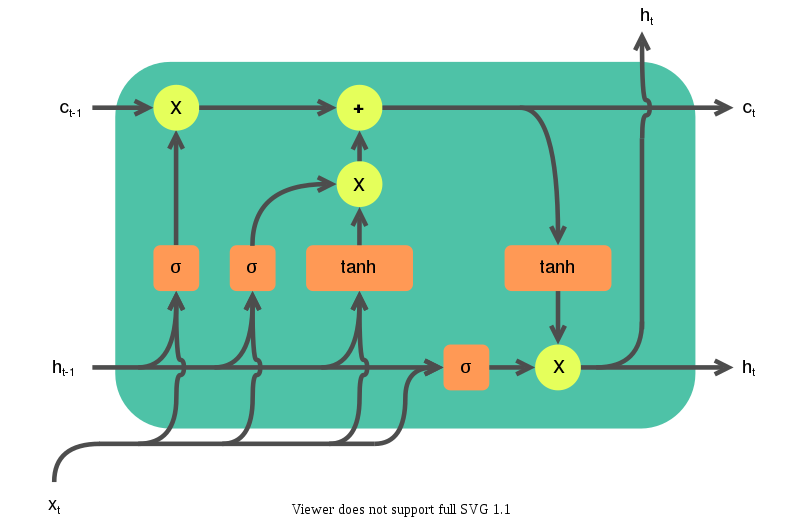
\includegraphics[width=0.6\textwidth]{resources/LSTM/LSTM_cell.png}
    \caption{Satu sel LSTM}
\end{figure}

LSTM Autoencoder adalah model neural network yang menggunakan LSTM sebagai hidden layernya untuk belajar menyalin input ke output. Autoencoder terdiri dari dua bagian, yaitu encoder yang menyalin input menjadi kode dan decoder yang menyalin kode menjadi output.

\begin{figure}[h]
    \centering
    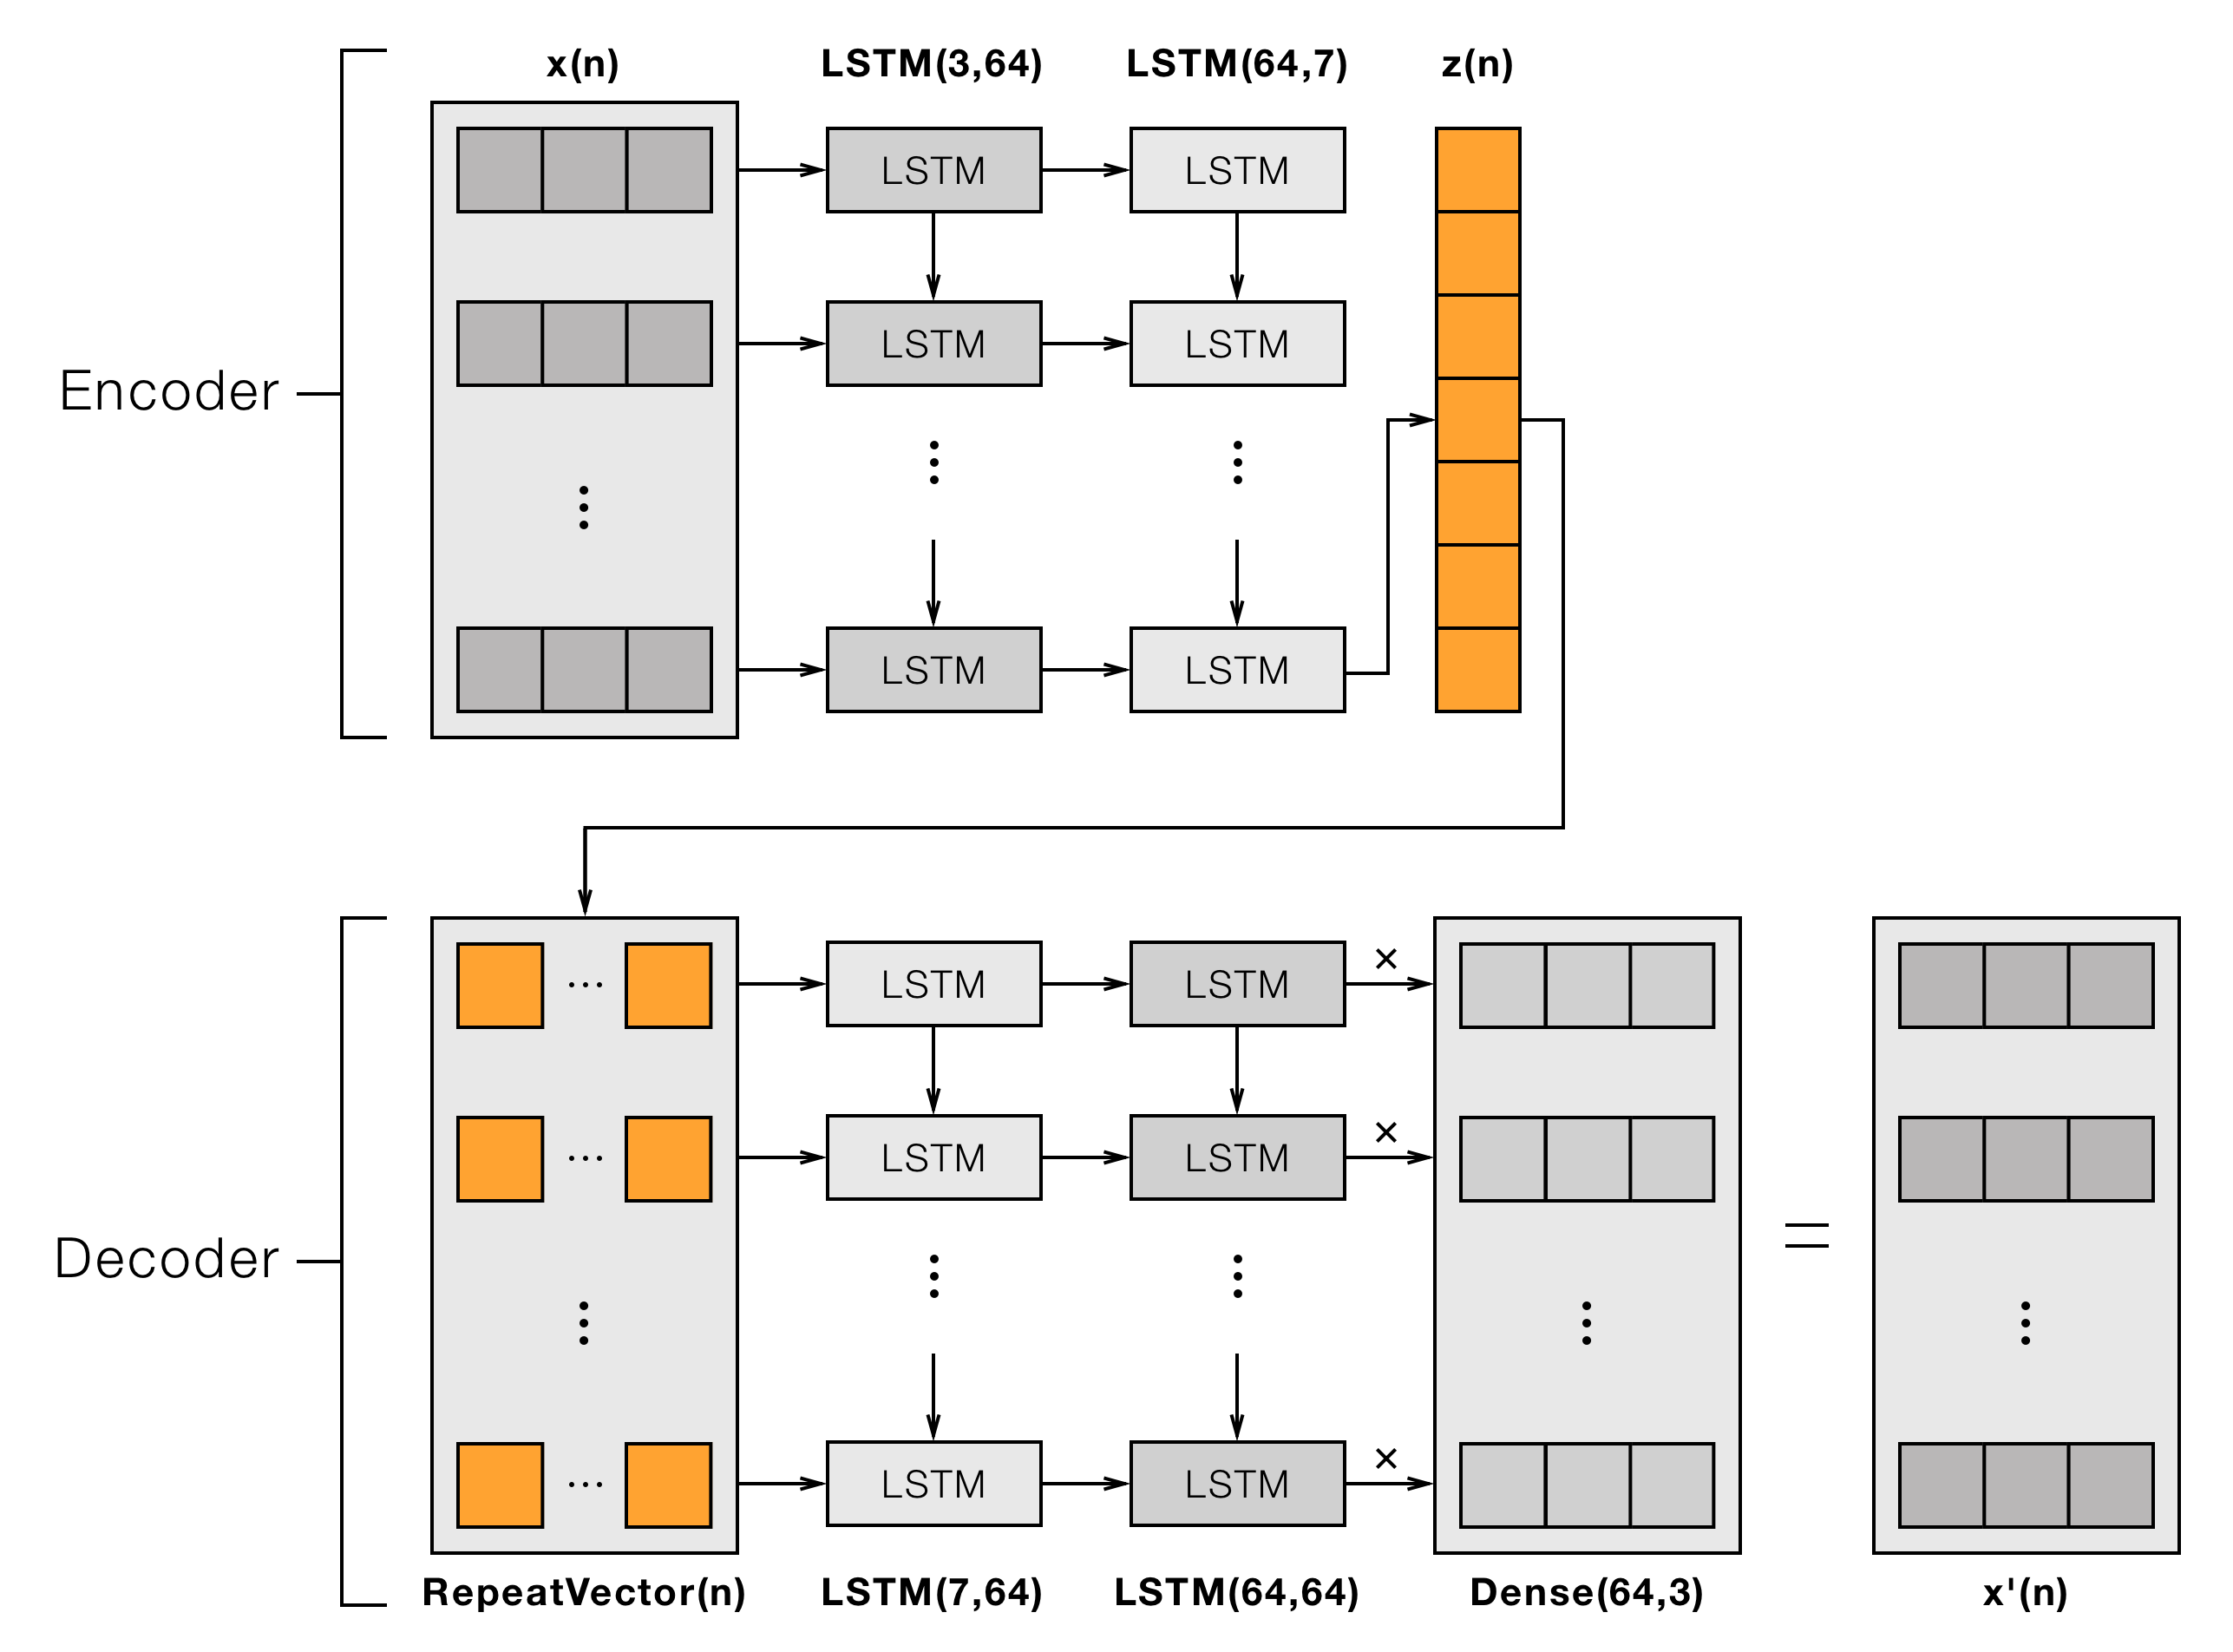
\includegraphics[width=0.8\textwidth]{resources/LSTM/lstm_ae.png}
    \caption{LSTM Autoencoder}
\end{figure}

Dengan begitu autoencoder dapat mempelajari fitur-fitur yang dimiliki input sehingga dapat melakukan prediksi, dan jika menggunakan LSTM sebagai hidden layernya maka dapat digunakan untuk memprediksi input berupa time series.

Karena lebih cocok untuk data time series, maka diharapkan model ini mampu memberikan hasil lebih baik dari model acuan.

Model LSTM Autoencoder didefinisikan melalui class \texttt{Encoder} dan \texttt{Decoder} yang kemudian digabung pada class \texttt{RecurrentAutoencoder} \cite{lstm}. Algoritma python untuk model LSTM Autoencoder dapat dilihat pada \ref{lstm_pca_ipynb} untuk model LSTM dengan PCA, dan \ref{lstm_nopca_ipynb} untuk model LSTM tanpa PCA.

\section{Bayesian Probability}
\subsection{Ide, Konsep, dan Hipotesis}

Ide awal untuk menggunakan model Bayesian untuk anomaly detection berasal dari konsep anomaly detection menggunakan pendekatan identifikasi data outlier. Beberapa metode umum untuk mendeteksi data outlier seperti K-Means Clustering dan Isolation Forest menggunakan konsep pengelompokkan data atau clustering data. Sehingga akan diperoleh data-data yang berada didalam cluster tersebut dan data yang berada diluar cluster diidentifikasi sebagai outlier.

\begin{figure}[h]
    \centering
    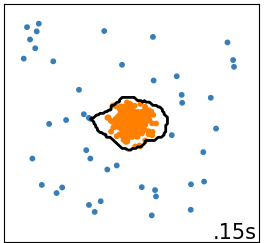
\includegraphics[width=200px]{resources/Bayes/isoforest.png}
    \caption{Isolation Forest Clustering}
\end{figure}

\begin{figure}[h]
    \centering
    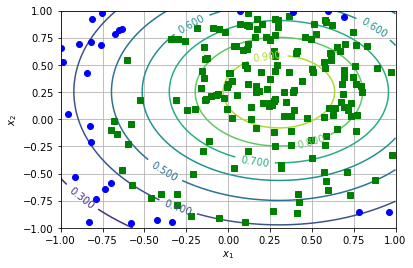
\includegraphics[width=200px]{resources/Bayes/bayes_model.png}
    \caption{Bayesian model untuk respon biner}
\end{figure}

Terlihat disini bahwa pendekatan clustering ini mirip dengan model Bayesian untuk respon biner. Asumsikan setiap data memiliki suatu probabilitas apakah data tersebut termasuk pada cluster normal ataukah outlier. Dengan begitu, dapat diekspektasi distribusi probabilitas akan memiliki kontur lingkaran. Semakin dekat suatu data dengan pusat lingkaran, maka data tersebut semakin likely merupakan data normal. Pusat lingkaran akan menjadi titik dengan probabilitas suatu data merupakan data normal sebesar 1, artinya pusat lingkaran adalah titik data ideal dari kondisi normal dataset, dalam kasus ini yaitu hasil pengukuran ideal dari sensor-sensor pada sistem mesin. Sebaliknya, semakin jauh dari pusat lingkaran maka akan semakin unlikely data tersebut adalah data normal, atau dalam arti lain: data tersebut semakin likely merupakan anomaly.

Hipotesis penulis terhadap model ini adalah model dapat dengan mudah mendeteksi anomaly ketika data tersebut outlier atau jauh dari data normal lain. Anomaly yang terjadi pada pinggiran cluster normal akan memiliki kemungkinan terdeteksi dan tidak, bergantung pada threshold yang digunakan. Namun model akan sulit mendeteksi anomaly yang berada ditengah-tengah kumpulan data normal.

\subsection{Deriving the Maths}

Definisikan data yang menjadi input model ini adalah 2 komponen utama dari hasil Principal Componen Analysis (PCA). Hal ini karena semakin tinggi dimensi data input, model akan semakin kompleks. Oleh karena itu data yang akan digunakan adalah komponen pertama PCA (pc1) sebagai $x_0$ dan komponen kedua PCA (pc2) sebagai $x_1$.

\begin{equation}
    \mathbf{x_n}=\begin{bmatrix} x_0 \\ x_1 \end{bmatrix}
\end{equation}

Sesuai ekspektasi awal, distribusi probabilitas akan memiliki kontur lingkaran. Maka, diperlukan 2 buah fungsi. Pertama adalah fungsi yang memetakan $\mathbf{x_n}$ ke suatu nilai dengan kontur lingkaran. Kedua adalah fungsi yang memetakan nilai kontur tersebut ke dalam range $[0,1]$, karena probabilitas hanya bernilai diantara 0 hingga 1.

Definisikan fungsi pertama sebagai
\begin{equation}
    f(\mathbf{w,x_n})=(w_0+x_0)^2+(w_1+x_1)^2 \label{fungsi_f}
\end{equation}
dengan
\begin{equation}
    \mathbf{w}=\begin{bmatrix} w_0 \\ w_1 \end{bmatrix}
\end{equation}
sebagai vektor parameter yang menentukan bentuk dan posisi kontur. Kemudian, dengan menetapkan data normal memiliki respon $t_n=1$ dan data anomaly memiliki respon $t_n=0$, didefinisikan fungsi kedua sebagai
\begin{equation*}
    P(T_n=1|\mathbf{x_n}, \mathbf{w}) = \frac{1}{1+f(\mathbf{w,x_n})}
\end{equation*}
Untuk penyederhanaan penulisan, $f(\mathbf{w,x_n})$ akan disingkat sebagai $f$ dan $P(T_n=1|\mathbf{x_n}, \mathbf{w})$ sebagai $P_n$.
\begin{equation}
    P_n = \frac{1}{1+f} \label{Pn}
\end{equation}
Konsep model bayesian menggunakan pendekatan dengan memisalkan suatu sampling dengan rasio sukses $p = P(T_n=1|\mathbf{x_n},\mathbf{w})$, sampling dilakukan hanya 1 kali ($N=1$) untuk total sukses sebanyak $Y_N=t_n$. Maka dengan distribusi binomial
\begin{align*}
    P(T_n=t_n|\mathbf{x_n},\mathbf{w})&=\mathbf{Binomial}(Y_N=y|p,N)\\
    &=\frac{N!}{(N-y)!y!}p^{y}(1-p)^{N-y}\\
    &=P(T_n=1|x_n,w)^{t_n}\left(1-P(T_n=1|x_n,w)\right)^{1-t_n}\\
    &=P_n^{t_n}\left(1-P_n)\right)^{1-t_n} \numberthis \label{likelihood}
\end{align*}
Berdasarkan data yang diketahui ($\mathbf{x_n}$ dan $t_n$), dengan asumsi seluruh data saling independen, dapat dihitung probability likelihood sebagai
\begin{equation*}
    p(t|\mathbf{X},\mathbf{w})=\prod_{n=1}^{N} P(T_n=t_n|\mathbf{x_n},\mathbf{w})
\end{equation*}
\begin{equation}
    p(t|\mathbf{X},\mathbf{w})=\prod_{n=1}^{N} P_n^{t_n}\left(1-P_n)\right)^{1-t_n}
\end{equation}
Persamaan probabilitas bayes adalah
\begin{equation}
    p(\mathbf{w}|\mathbf{X},t)=\frac{p(t|\mathbf{X},\mathbf{w})p(\mathbf{w})}{p(t|\mathbf{X})}
\end{equation}
Pada kasus anomaly detection, model dilatih untuk mencari parameter $\mathbf{w}$ yang terbaik dalam memetakan seluruh data yang diasumsikan data normal sebagai data yang likely merupakan data normal. Model bayesian memodelkan seluruh variabel sebagai variabel bebas yang terdistribusi dengan suatu probabilitas. Maka, parameter $\mathbf{w}$ yang terbaik adalah ekspektasi dari distribusi probabilitas $p(\mathbf{w}|\mathbf{X},t)$. Sehingga, parameter $\mathbf{w}$ terbaik akan berada pada titik maksimum dari $p(\mathbf{w}|\mathbf{X},t)$. Oleh karena itu, $\mathbf{w}$ terbaik dapat ditentukan dengan menyelesaikan
\begin{equation*}
    \frac{\partial{p(\mathbf{w}|\mathbf{X},t)}}{\partial{\mathbf{w}}} = 0
\end{equation*}
\begin{equation*}
    \frac{\partial}{\partial{\mathbf{w}}} \frac{p(t|\mathbf{X},\mathbf{w})p(\mathbf{w})}{p(t|\mathbf{X})} = 0
\end{equation*}
Karena $p(t|\mathbf{X})$ independen terhadap $\mathbf{w}$, Maka
\begin{equation}
    \frac{\partial}{\partial{\mathbf{w}}} p(t|\mathbf{X},\mathbf{w})p(\mathbf{w}) = 0 \label{ODE}
\end{equation}
Asumsikan parameter $\mathbf{w}$ terdistribusi normal
\begin{equation}
    p(\mathbf{w})=\mathcal{N}_\mathbf{w}\left(0,\sigma^2\mathbf{I}\right)=\mathcal{N}_{w_1}\left(0,\sigma^2\right)\mathcal{N}_{w_2}\left(0,\sigma^2\right) \label{prior}
\end{equation}
Maka, dari persamaan \ref{likelihood} dan \ref{prior}, persamaan \ref{ODE} menjadi
\begin{equation}
    \frac{\partial{}}{\partial{\mathbf{w}}} \left(p(\mathbf{w})\prod_{n=1}^{N} P_n^{t_n}\left(1-P_n\right)^{1-t_n}\right)=0
\end{equation}
Persamaan ini sulit diselesaikan. Namun dengan mengambil logaritma natural kedua sisi akan diperoleh
\begin{equation*}
    \frac{\partial{}}{\partial{\mathbf{w}}} \left(\ln{\left[p(\mathbf{w})\prod_{n=1}^{N} P_n^{t_n}\left(1-P_n\right)^{1-t_n}\right]}\right)=0
\end{equation*}
\begin{equation}
    \frac{\partial{}}{\partial{\mathbf{w}}}\left(\ln{\left[ p(\mathbf{w}) \right]}\right) + \frac{\partial{}}{\partial{w}} \left(\ln{\left[ \prod_{n=1}^{N} P_n^{t_n}\left(1-P_n\right)^{1-t_n}\right] }\right)=0
\end{equation}
Untuk suku pertama:
\begin{equation*}
\ln{\left[ p(\mathbf{w}) \right]} = \ln{\left[ \mathcal{N}_{w_1}\left(0,\sigma^2\right)\mathcal{N}_{w_2}\left(0,\sigma^2\right) \right]}
\end{equation*}
\begin{equation*}
\ln{\left[ p(\mathbf{w}) \right]}=\ln{\left[ \frac{1}{\sqrt{2\pi\sigma^2}}e^{-\frac{w_1^2}{2\sigma^2}} \frac{1}{\sqrt{2\pi\sigma^2}}e^{-\frac{w_2^2}{2\sigma^2}} \right]}
\end{equation*}
\begin{equation*}
\ln{\left[ p(\mathbf{w}) \right]}=-\frac{w_1^2+w_2^2}{2\sigma^2}-\ln\left({2\pi\sigma^2}\right)
\end{equation*}
\begin{equation}
\frac{\partial{}}{\partial{\mathbf{w}}}\left(\ln{\left[ p(\mathbf{w}) \right]}\right)=-\frac{\mathbf{w^T}}{\sigma^2} \label{ODE_1st_term}
\end{equation}

dan untuk suku kedua:
\begin{equation*}
    \ln{\left[ \prod_{n=1}^{N} P_n^{t_n}\left(1-P_n\right)^{1-t_n} \right] }=\sum_{n=1}^{N} \ln{ \left[ P_n^{t_n}\left(1-P_n\right)^{1-t_n} \right] }
\end{equation*}
\begin{equation*}
    \ln{\left[ \prod_{n=1}^{N} P_n^{t_n}\left(1-P_n\right)^{1-t_n} \right] }=\sum_{n=1}^{N} t_n\ln{(P_n)} + (1-t_n)\ln{(1-P_n)}
\end{equation*}
Variabel $t_n$ adalah data yang diketahui dari dataset, ini berarti $t_n$ independen dari $\mathbf{w}$. Sehingga:
\begin{equation}
    \frac{\partial}{\partial{\mathbf{w}}} \ln{\left[ \prod_{n=1}^{N} P_n^{t_n}\left(1-P_n\right)^{1-t_n} \right] } = \sum_{n=1}^{N} t_n \frac{\partial}{\partial{\mathbf{w}}}\ln{(P_n)} + (1-t_n) \frac{\partial}{\partial{\mathbf{w}}} \ln{(1-P_n)} \label{ODE_2nd_term}
\end{equation}
Selesaikan dahulu suku $\frac{\partial{P_n}}{\partial{\mathbf{w}}}$
\begin{equation*}
    \frac{\partial{P_n}}{\partial{\mathbf{w}}} = \frac{\partial{P_n}}{\partial{f}} \frac{\partial{f}}{\partial{\mathbf{w}}} = \frac{\partial}{\partial{f}} \left( \frac{1}{1+f} \right) \frac{\partial{f}}{\partial{\mathbf{w}}}
\end{equation*}
Definisikan suatu fungsi $g(f)$ sebagai
\begin{equation}
    g(f) = \frac{\partial}{\partial{f}} \left( \frac{1}{1+f} \right) = -\frac{1}{(1+f)^2} \label{fungsi_g}
\end{equation}
Untuk mempersingkat penulisan, fungsi $g(f)$ akan disingkat menjadi $g$. Diperoleh
\begin{equation}
    \frac{\partial{P_n}}{\partial{\mathbf{w}}} = g \frac{\partial{f}}{\partial{\mathbf{w}}} \label{dPndw_vec}
\end{equation}
dengan
\begin{equation}
    \frac{\partial{f}}{\partial{\mathbf{w}}} = \begin{bmatrix} \frac{\partial{f}}{\partial{w_0}} && \frac{\partial{f}}{\partial{w_1}}\end{bmatrix} \label{dfdw_vec}
\end{equation}
dan dari persamaan \ref{fungsi_f}, dapat diperoleh
\begin{equation}
    \frac{\partial{f}}{\partial{w_i}} = 2(w_i+x_i) \label{dfdwn}
\end{equation}
serta komponen-komponen pada vektor $\frac{\partial{P_n}}{\partial{\mathbf{w}}}$ menjadi
\begin{equation}
    \frac{\partial{P_n}}{\partial{w_i}} = g \frac{\partial{f}}{\partial{w_i}} \label{dPndwn}
\end{equation}
Maka, dengan persamaan \ref{dPndw_vec} persamaan \ref{ODE_2nd_term} menjadi
\begin{align*}
    \frac{\partial}{\partial{\mathbf{w}}} \ln{\left[ \prod_{n=1}^{N} P_n^{t_n}\left(1-P_n\right)^{1-t_n} \right] } & = \sum_{n=1}^{N} t_n \frac{\partial}{\partial{\mathbf{w}}}\ln{(P_n)} + (1-t_n) \frac{\partial}{\partial{\mathbf{w}}} \ln{(1-P_n)} \\
    & = \sum_{n=1}^{N} t_n \frac{1}{P_n} \frac{\partial{P_n}}{\partial{\mathbf{w}}} - (1-t_n) \frac{1}{(1-P_n)} \frac{\partial{P_n}}{\partial{\mathbf{w}}} \\
    & = \sum_{n=1}^{N} t_n \frac{1}{P_n} g \frac{\partial{f}}{\partial{\mathbf{w}}} - (1-t_n) \frac{1}{(1-P_n)} g \frac{\partial{f}}{\partial{\mathbf{w}}} \\
    & = \sum_{n=1}^{N} \frac{(t_n-P_n)g}{P_n(1-P_n)} \frac{\partial{f}}{\partial{\mathbf{w}}} \numberthis \label{ODE_2nd_term_2}
\end{align*}
Dengan persamaan \ref{ODE_1st_term} dan \ref{ODE_2nd_term_2} didapatkan persamaan \ref{ODE} menjadi
\begin{equation}
    -\frac{\mathbf{w^T}}{\sigma^2}+\sum_{n=1}^{N} \frac{(t_n-P_n)g}{P_n(1-P_n)} \frac{\partial{f}}{\partial{\mathbf{w}}}=0 \label{ODE_final}
\end{equation}
Persamaan ini tidak dapat diselesaikan secara analitik. Namun dengan metode numerik Newton-Rhapson, solusi $\mathbf{w}$ dapat diperoleh dengan mendefinisikan
\begin{equation}
    \mathbf{F^T}(\mathbf{w}) = -\frac{\mathbf{w^T}}{\sigma^2}+\sum_{n=1}^{N} \frac{(t_n-P_n)g}{P_n(1-P_n)} \frac{\partial{f}}{\partial{\mathbf{w}}} \label{F_vec}
\end{equation}
Maka persamaan \ref{ODE_final} terpenuhi pada kondisi $\mathbf{F^T}(\mathbf{w}) = 0$ yang dapat ditentukan dengan menebak suatu $\mathbf{w}$ awal dan melakukan iterasi
\begin{equation}
    \mathbf{w}_{i+1} = \mathbf{w}_{i} - \mathbf{H}^{-1}\mathbf{F}(\mathbf{w}) \label{iter}
\end{equation}
Dengan $\mathbf{H}$ adalah Hessian matrix
\begin{equation}
    \mathbf{H} = 
    \begin{bmatrix}
    \frac{\partial{F_0}}{\partial{w_0}} & \frac{\partial{F_0}}{\partial{w_1}} \\
    \frac{\partial{F_1}}{\partial{w_0}} & \frac{\partial{F_1}}{\partial{w_1}} 
    \end{bmatrix} \label{H_mat}
\end{equation}
dan $F_0$ serta $F_1$ adalah komponen-komponen dari vektor $\mathbf{F}(\mathbf{w})$. Elemen-elemen pada matrix hessian dapat ditentukan dengan
\begin{align*}
    \frac{\partial{F_j}}{\partial{w_i}} =& - \frac{\delta_{ij}}{\sigma^2} + \sum_{n=1}^{N}
    \left[
        \frac{(t_n-P_n)g}{P_n(1-P_n)} \frac{\partial^2{f}}{\partial{w_i}\partial{w_j}}
    \right] \\
    &+ \sum_{n=1}^{N}
    \left[
    \left(
    \frac{
    (t_n-P_n) \frac{\partial{g}}{\partial{w_i}} - g \frac{\partial{P_n}}{\partial{w_i}}
    }{P_n(1-P_n)}
    - \frac{(t_n-P_n)g}{P_n^2(1-P_n)^2} (1-2P_n) \frac{\partial{P_n}}{\partial{w_i}}
    \right)
    \frac{\partial{f}}{\partial{w_j}}
    \right]
    \numberthis \label{dFn_dwm}
\end{align*}
dengan $\delta_{ij}$ adalah fungsi delta kronecker. Kemudian persamaan \ref{fungsi_g} dan \ref{fungsi_f} dapat diperoleh
\begin{equation}
    \frac{\partial{g}}{\partial{w_i}} = \frac{1}{(1+f)^3} \frac{\partial{f}}{\partial{w_i}} \label{dotg}
\end{equation}
\begin{equation}
    \frac{\partial^2{f}}{\partial{w_i}\partial{w_j}} = 2\delta_{ij} \label{ddotf}
\end{equation}


\subsection{Algorithma}

Model bayesian hanya didefinisikan dengan array yang mewakili parameter $\mathbf{w}$. Kemudian model training dilakukan dengan meng-iterasi $\mathbf{w}$ menggunakan persamaan \ref{iter} hingga hasil iterasi konvergen. Kemudian hasil parameter $\mathbf{w}$ digunakan kembali untuk persamaan \ref{Pn} dan \ref{fungsi_f} dengan input test data. Probabilitas suatu data merupakan data normal dari seluruh test data akan diperoleh. Algoritma python model Bayesian dapat dilihat pada \ref{bayes_ipynb}.

    \chapter{Analisis}

\section{LSTM Autoencoder}

Data dipisah menjadi dua bagian, yaitu data normal yang mengandung data dari status NORMAL dan data anomali yang berasal dari status selain NORMAL (BROKEN dan RECOVERY).

Kemudian data dibagi menjadi 3 dataset, yaitu train, validation, dan test. Data train dan validation diambil pada bulan ke-8 awal dan akhir masing-masing dan digunakan untuk training model, sedangkan data test diambil pada selain bulan ke-8 untuk memprediksi hasil anomali.

Proses training model LSTM Autoencoder dilakukan sebanyak 5 epoch yang memakan waktu sekitar 20 menit. Data train dan validation dibagi menjadi dua macam, yaitu yang telah menggunakan PCA dan tanpa PCA.

Kemudian dilakukan prediksi pada data test dari model yang telah dilakukan training sehingga dapat diperoleh nilai loss yang dihasilkan.

    \subsection{Dengan PCA}

    \begin{figure}[h]
        \centering
        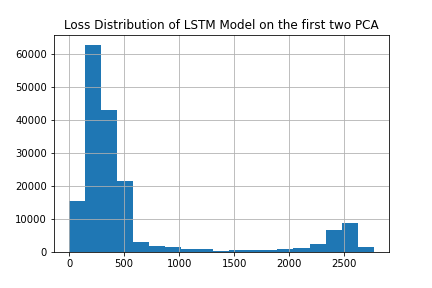
\includegraphics[width=0.8\textwidth]{resources/LSTM/LSTM_PCA_LossDist.png}
        \caption{Distribusi loss LSTM dengan PCA}
    \end{figure}

    Dengan menggunakan nilai threshold 500, diperoleh jumlah data anomali sebagai berikut.

    \begin{table}[h]
        \centering
        \begin{tabular}{|l|r|r|r|}
            \hline
            \multicolumn{1}{|c|}{\textbf{Jenis anomali}} & \multicolumn{1}{c|}{\textbf{Jumlah}} & \multicolumn{1}{c|}{\textbf{Total data}} & \multicolumn{1}{c|}{\textbf{Persentase (\%)}} \\ \hline
            Anomali pada data NORMAL                     & 33866                                & 160430                                   & 21                                       \\ \hline
            Anomali pada data selain NORMAL              & 2237                                 & 14454                                    & 15                                       \\ \hline
        \end{tabular}
    \end{table}

    Jumlah anomali pada data selain NORMAL tidak mencakup keseluruhan total data sehingga terdapat prediksi yang berada pada data dalam kondisi BROKEN atau RECOVERY.

    \subsection{Tanpa PCA}

    \begin{figure}[h]
        \centering
        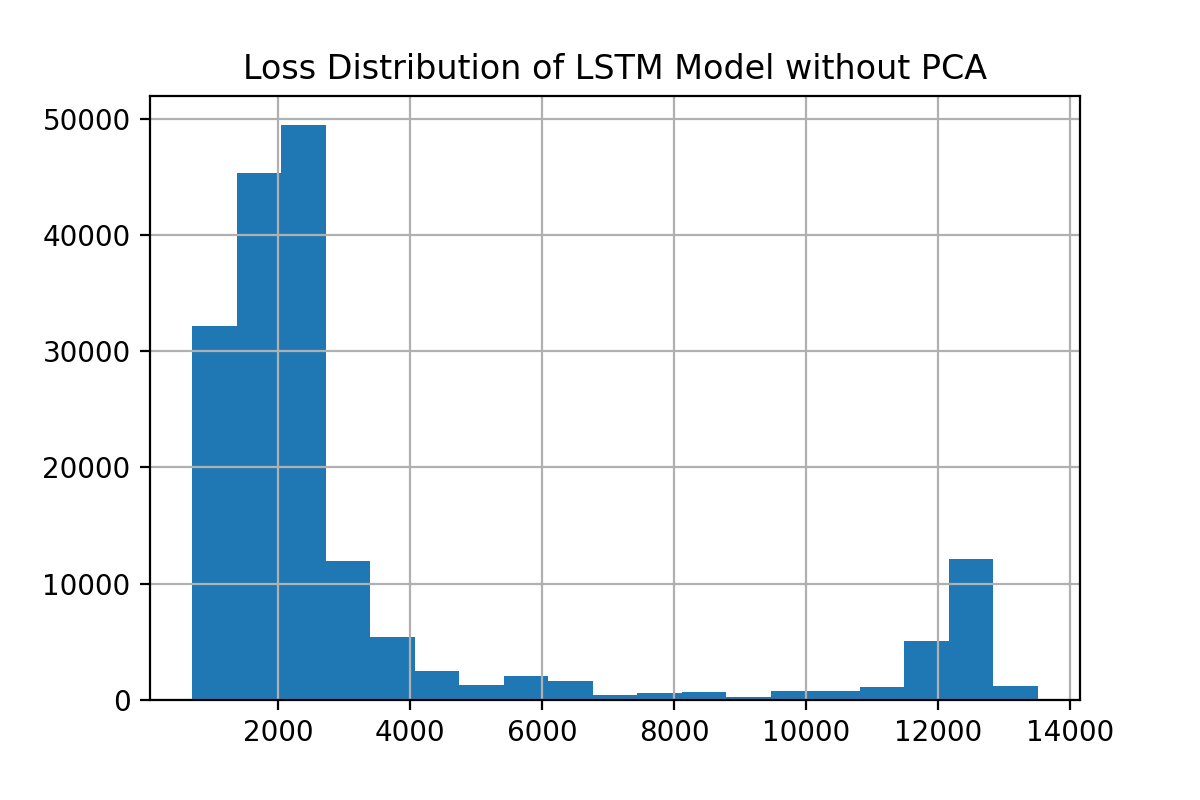
\includegraphics[width=0.8\textwidth]{resources/LSTM/LSTM_noPCA_LossDist.png}
        \caption{Distribusi loss LSTM tanpa PCA}
    \end{figure}

    Dengan menggunakan nilai threshold 3500, diperoleh jumlah data anomali sebagai berikut.

    \begin{table}[h]
        \centering
        \begin{tabular}{|l|r|r|r|}
            \hline
            \multicolumn{1}{|c|}{\textbf{Jenis anomali}} & \multicolumn{1}{c|}{\textbf{Jumlah}} & \multicolumn{1}{c|}{\textbf{Total data}} & \multicolumn{1}{c|}{\textbf{Persentase (\%)}} \\ \hline
            Anomali pada data NORMAL                     & 30182                                & 160430                                   & 19                                       \\ \hline
            Anomali pada data selain NORMAL              & 4979                                 & 14454                                    & 34                                       \\ \hline
        \end{tabular}
    \end{table}

    Terlihat bahwa jumlah anomali pada data NORMAL lebih sedikit 3\% dari analisis dengan PCA, Namun jumlah anomali pada data selain NORMAL juga meningkat hampir 2 kali lipat.

    \chapter{Penutup}

\section{Kesimpulan}
Berdasarkan analisis pada hasil prediksi anomaly keenam model seperti pada \ref{ANALISIS}, disimpulkan:
\begin{enumerate}
    \item Model kembangan unggul dalam mendeteksi kerusakan pada bulan-bulan awal, namun model acuan unggul pada bulan-bulan akhir.
    \item Model kembangan LSTM Autoencoder berhasil mendeteksi anomali yang overlap dengan data normal.
    \item Model terbaik adalah LSTM Autoencoder dengan PCA dalam kriteria keberhasilan memprediksi kerusakan mesin dan \emph{false positive rate}.
\end{enumerate}

\section{Saran}

Masih banyak metode dan model lain yang dapat digunakan dalam kasus anomaly detection. Tidak hanya itu saja, tahap preprocessing data juga dapat berpenguh pada performa model. Kemudian, banyak faktor-faktor luar yang tidak terkandung dalam data yang dapat mempengaruhi \emph{model learning}, contohnya maintenance mesin tak terjadwal yang mungkin dilakukan oleh pemilik mesin. Durasi maintenance mesin yang berubah-ubah juga dapat membuat model sulit mengenali anomali. Kerusakan yang tidak diakibatkan oleh kesalahan internal mesin juga mungkin terjadi, misalnya kerusakan mesin akibat \emph{human error}, ini akan menyebabkan kerusakan mendadak tanpa terdeteksi anomali sebelum kerusakan terjadi.

Dengan begitu, tidak ada suatu metode eksak yang terbaik dalam anomaly detection. Yang ada hanyalah model yang paling cocok pada suatu mesin untuk memprediksi kerusakan. Seberapa \emph{severe} kerusakan yang dapat terjadi juga menjadi pertimbangan, serta \emph{computational cost} yang dibutuhkan untuk melatih model.
    %----------------------------------------------------------------%

    % Daftar pustaka
    \printbibliography

    % Index
    %\appendix

    %\addcontentsline{toc}{part}{Lampiran}
    %\part*{Lampiran}

    %\chapter{Notebook}

Daftar file Jupyter Notebook yang penulis lampirkan terdapat pada link Google Drive berikut: \\
\url{https://drive.google.com/drive/folders/1mjf-hefWUkvGAlhulI-Cl-TQ22Q1rUwh}

Jupyter Notebook program acuan dan modifikasi:
\begin{enumerate}[label=\textbf{L.\arabic*}]
    \item \texttt{Time Series Anomaly Detection -  Steps 1 and 2.ipynb}
    \item \texttt{Time Series Anomaly Detection - Steps 3 to 5.ipynb}
    \item \texttt{Model\textunderscore Reference\textunderscore Result\textunderscore Analysis.ipynb} (modifikasi penulis) \label{refmodified_ipynb}
\end{enumerate}

Jupyter Notebook program kembangan:
\begin{enumerate}[label=\textbf{L.\arabic*}]
    \setcounter{enumi}{4}
    \item \texttt{LSTM\textunderscore ver3\textunderscore revB.ipynb} \label{lstm_pca_ipynb}
    \item \texttt{LSTM\textunderscore ver3\textunderscore revB\textunderscore Result\textunderscore Analysis.ipynb} \label{lstm_pca_res_ipynb}
    \item \texttt{LSTM\textunderscore noPCA.ipynb} \label{lstm_nopca_ipynb}
    \item \texttt{LSTM\textunderscore noPCA\textunderscore Result\textunderscore Analysis.ipynb} \label{lstm_pca_res_ipynb}
    \item \texttt{Bayes\textunderscore revB.ipynb} \label{bayes_ipynb}
    \item \texttt{Bayes\textunderscore Result\textunderscore Analysis.ipynb} \label{lstm_pca_res_ipynb}
\end{enumerate}

    %\chapter{Grafik}

Beberapa grafik yang representatif. Lengkapnya terdapat pada link Google Drive pada lampiran sebelumnya.

\begin{figure}[h]
    %\centering
    \centerline{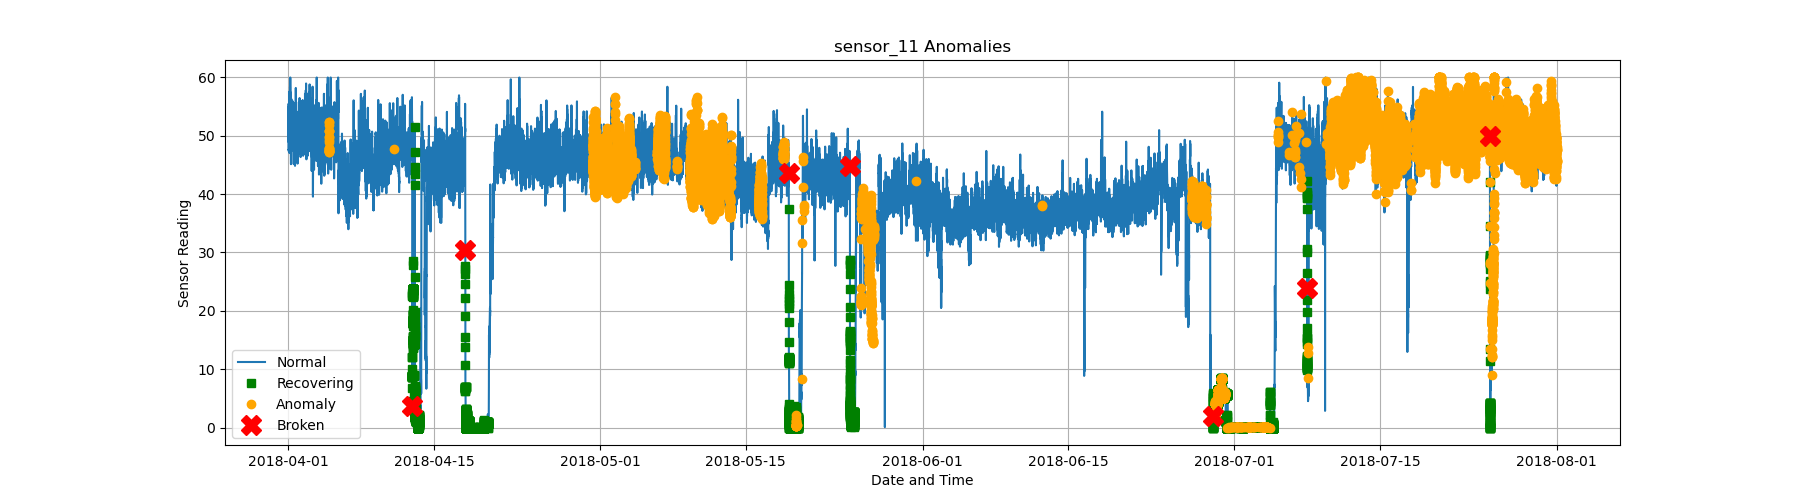
\includegraphics[width=1.4\textwidth]{resources/Acuan/IQR_sensor_11.png}}
    \caption{Hasil prediksi anomali model IQR} \label{IQR11}
\end{figure}
\begin{figure}[h]
    %\centering
    \centerline{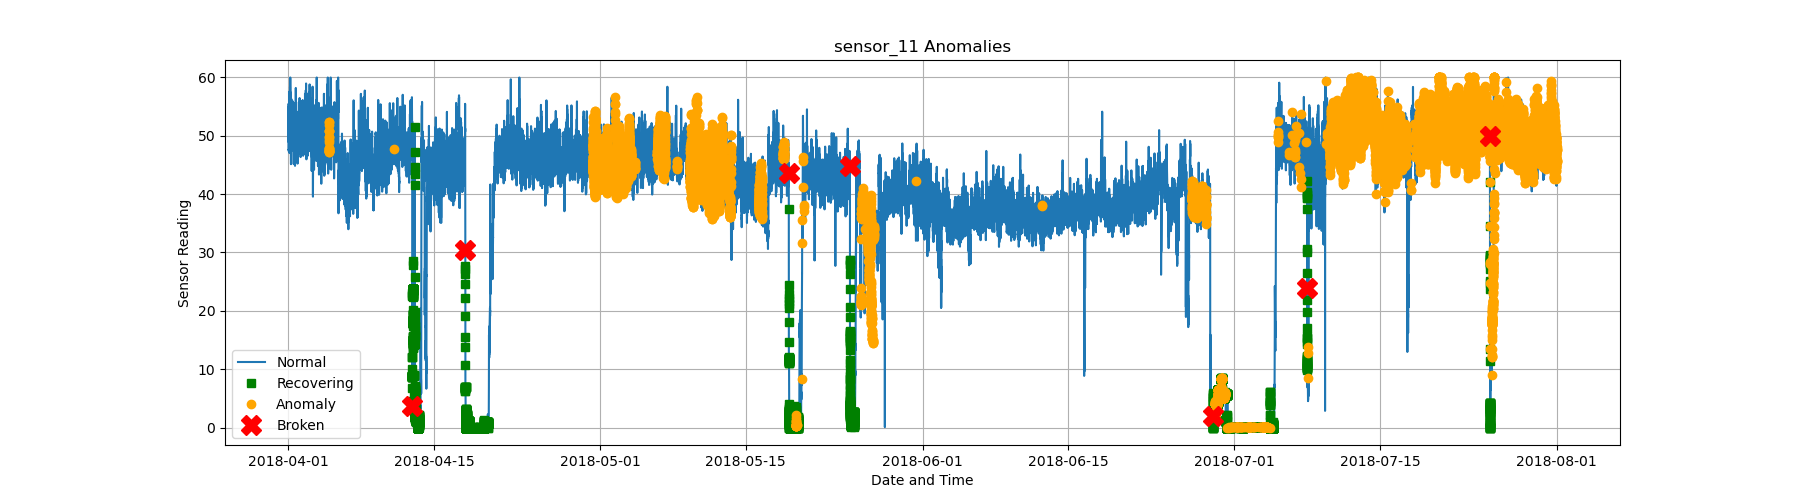
\includegraphics[width=1.4\textwidth]{resources/Acuan/KMeans_sensor_11.png}}
    \caption{Hasil prediksi anomali model K-Means Clustering} \label{KM11}
\end{figure}
\begin{figure}[h]
    %\centering
    \centerline{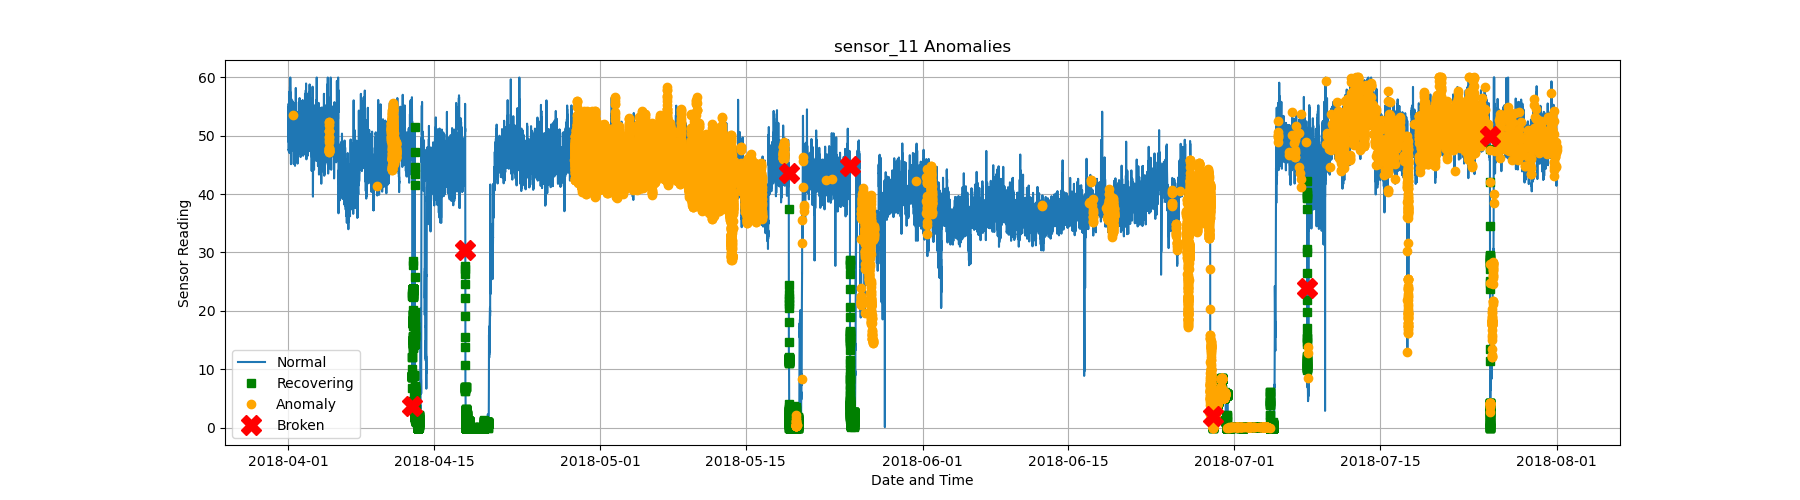
\includegraphics[width=1.4\textwidth]{resources/Acuan/IsoFor_sensor_11.png}}
    \caption{Hasil prediksi anomali model Isolation Forest} \label{IF11}
\end{figure}
\begin{figure}[h]
    %\centering
    \centerline{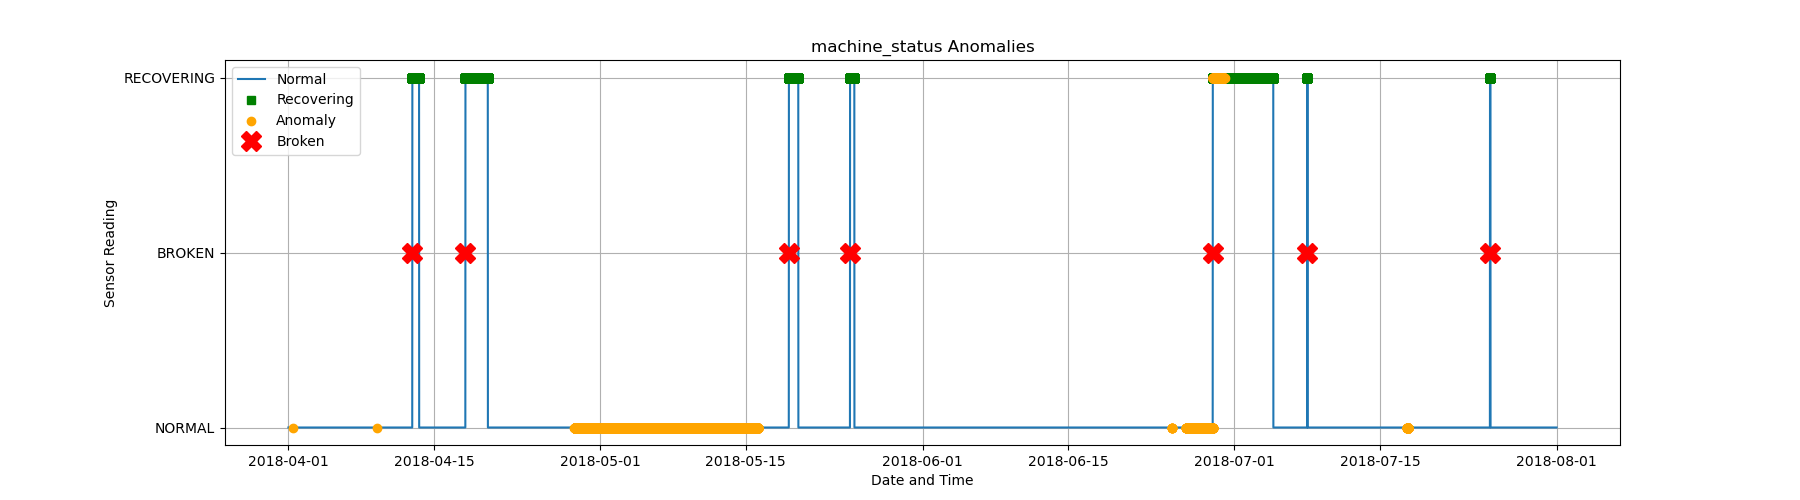
\includegraphics[width=1.4\textwidth]{resources/Acuan/IQR_machine_status.png}}
    \caption{Anomali model IQR dan status mesin} \label{IQRms}
\end{figure}
\begin{figure}[h]
    %\centering
    \centerline{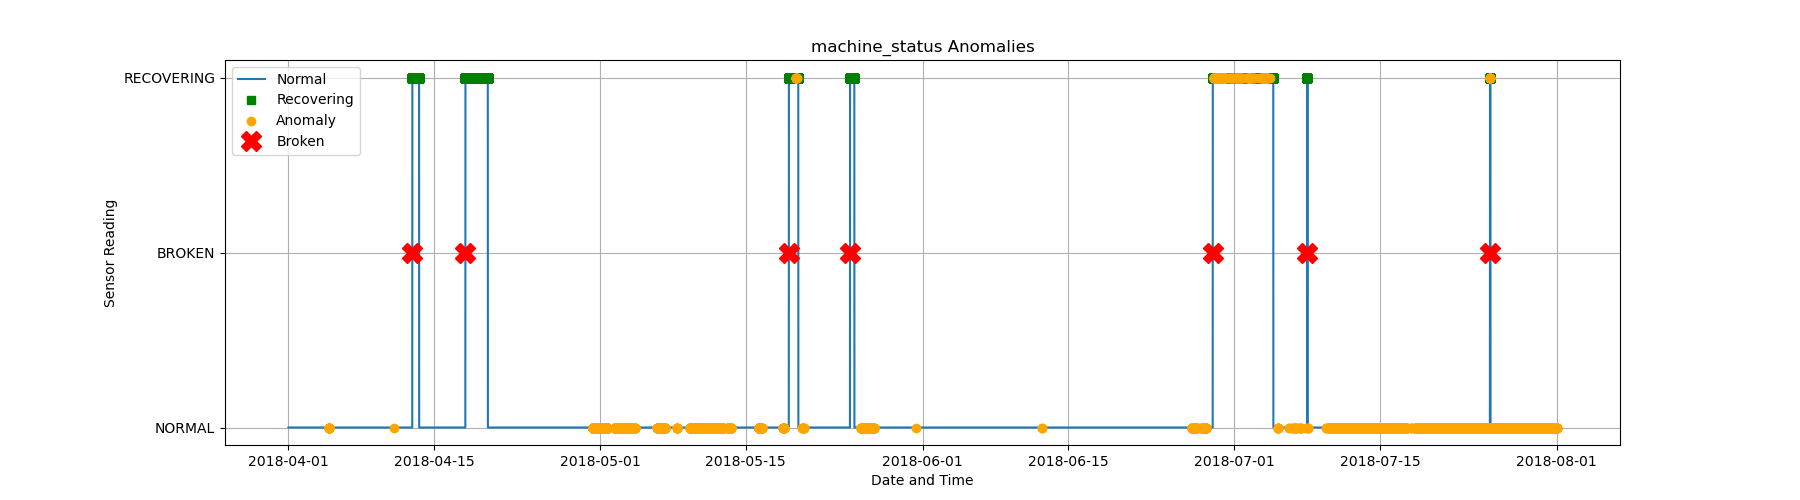
\includegraphics[width=1.4\textwidth]{resources/Acuan/KMeans_machine_status.png}}
    \caption{Anomali model K-Means Clustering dan status mesin} \label{KMms}
\end{figure}
\begin{figure}[h]
    %\centering
    \centerline{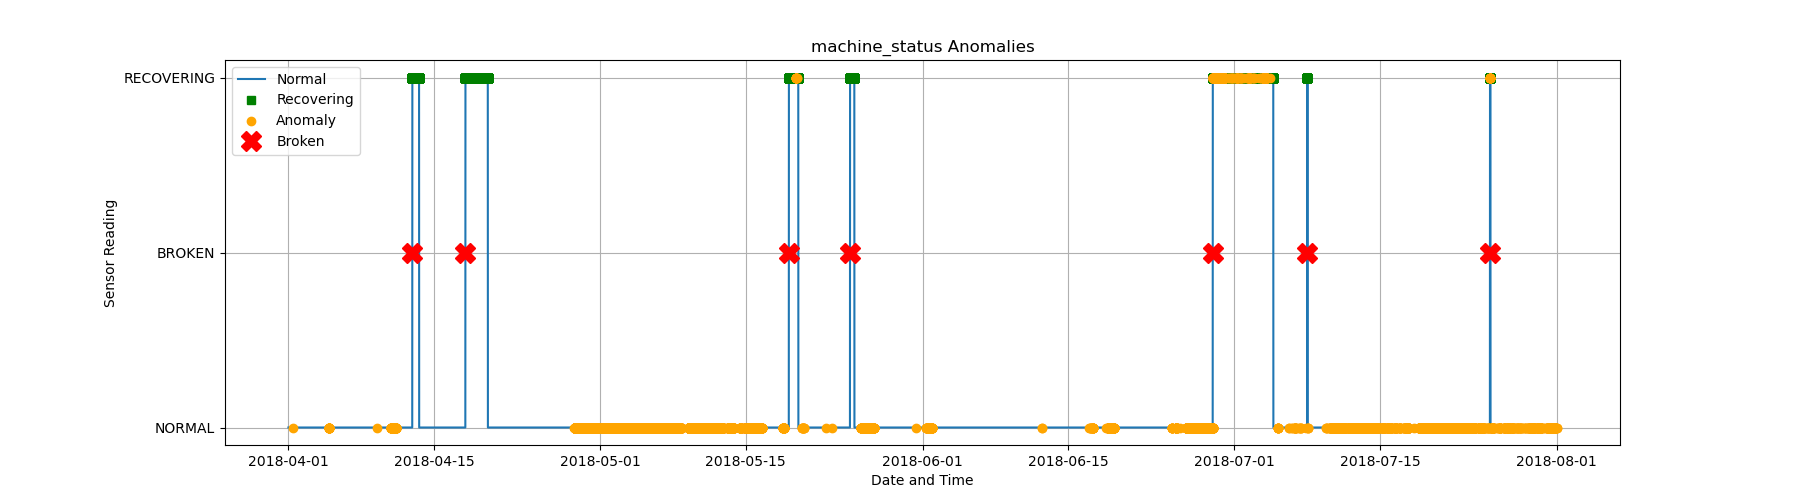
\includegraphics[width=1.4\textwidth]{resources/Acuan/IsoFor_machine_status.png}}
    \caption{Anomali model Isolation Forest dan status mesin} \label{IFms}
\end{figure}
\begin{figure}[h]
    %\centering
    \centerline{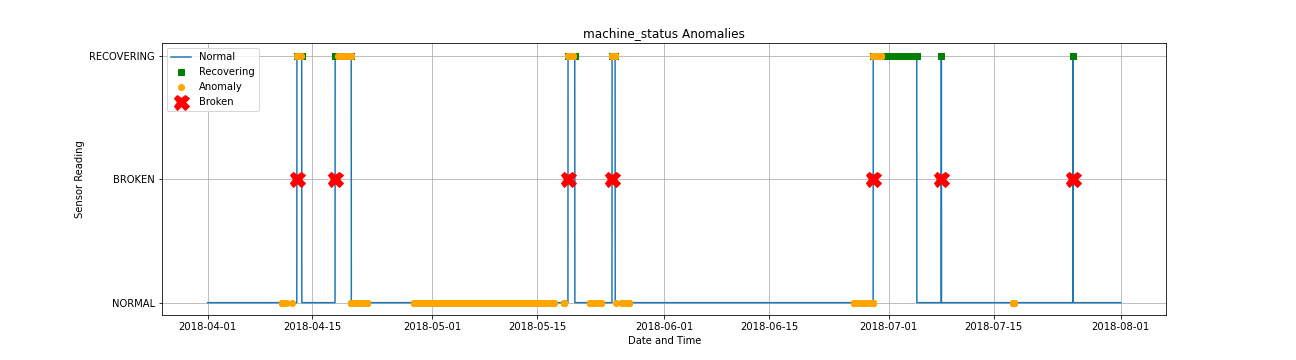
\includegraphics[width=1.4\textwidth]{resources/Bayes/Bayes_machine_status.png}}
    \caption{Anomali model Bayesian dan status mesin} \label{Bms}
\end{figure}
\begin{figure}[h]
    %\centering
    \centerline{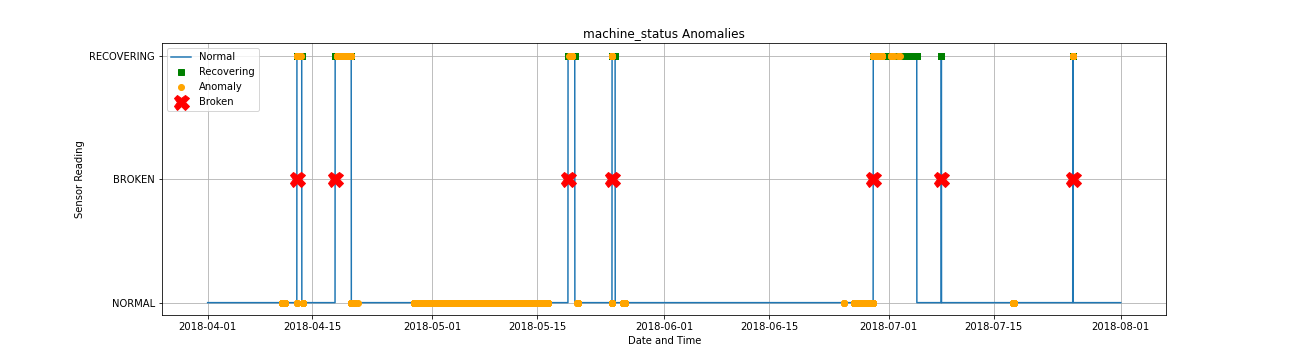
\includegraphics[width=1.4\textwidth]{resources/LSTM/LSTM_noPCA_machine_status.png}}
    \caption{Anomali model LSTM tanpa PCA dan status mesin} \label{nPms}
\end{figure}
\begin{figure}[h]
    %\centering
    \centerline{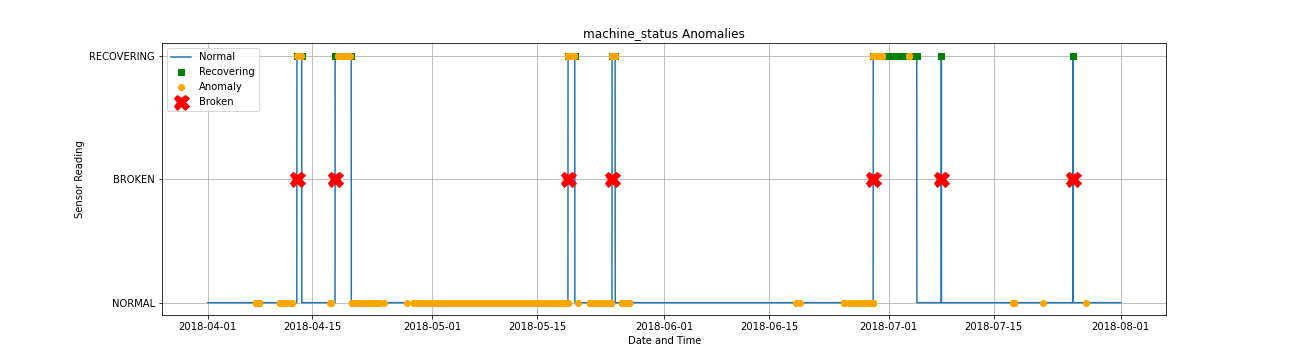
\includegraphics[width=1.4\textwidth]{resources/LSTM/LSTM_PCA_machine_status.png}}
    \caption{Anomali model LSTM dengan PCA dan status mesin} \label{wPms}
\end{figure}

\end{document}
